Studying Geometry one inadvertently meets a plethora of manifolds equipped with certain additional data or structure. 
Information like this can conveniently delt with in the framework of \emph{tangential structures}, which we shall explore in this Chapter.
We will see, how both \emph{orientations} and \emph{spin structures} arise as special cases of tangential structures, and will encounter a poweful invariant, the tangential $2$-type of a manifold, encoding richer nuances of these terms.\\
In a one page excerpt of Matthias Kreck's paper "Surgery and Duality" \cite{kreck:sad}, tangential types are defined and a classification of tangential $2$-types is given.
Since his writing style is rather dense and the proofs are at best sketches of the neccesary arguments, we take some time to stuff the theory with examples and comments, before giving a detailed proof of the mentioned classification result.
Our exploration irrelevantly differs from \cite{kreck:sad} by working with the (stable) tangent bundle instead of a stable normal Gauss Map.
The irrelevance of this choice is discussed in the great reference \cite{stong:cc}.\\
For a smooth reading experience, the reader should bring some knowledge of characteristic classes, classifying spaces of vector bundles, and stabilization of vectorbundles as is best obtained from the classic \cite{ms:cc} and can also be found in \cite{hatcher:vb}.
Furthermore a spoonful of maturity in the basic concepts of algebraic topology is required, all relevant concepts such as homotopy groups, homology and cohomology and universal coefficient theorems are for example discussed in \cite{hatcher:at}, \cite{ttd:at}, or \cite{may:at}.
We will especially also need some obstruction theory for fibrations, which can be also found in \cite{steenrod:fib}.
At one point we derive the exact sequence \hyperref[heartseq]{$\heartsuit$} using a spectral sequence argument, but the unfamiliar reader may skip this short digression without any fear of consequence.

\subsection{Notation and Conventions}
The term manifold and the symbol $M$ in this text refers always to a smooth, nonempty, compact, and connected manifold possibly with boundary if not explicitly stated otherwise. All our manifolds furthermore carry the datum of a fixed basepoint $p\in M$ and come with a given representative $\st\colon M \to \B\O$ that classifies their stable tangent bundle.
In the first part of chapter 2 we shortly divert from the assumptions of connectedness and nonemtpyness, but discuss at the end how to recover these assumptions.
Furthermore, there are of course some compact manifolds with noncompact universal covers, a problem which we wholeheartedly ignore for it will not matter in the cases which we will be interested in.\\
All other topological spaces $X$ also implicitly carry a fixed basepoint $x\in X$ and we write $\pi_k(X)$ without mentioning $x$ explicitly.
A space $X$ is called $k$-connected, if $\pi_i(X)$ vanishes for $i\leq k$, and $k$-coconnected, if it vanishes for $i\geq k$.
A continuous map of topological spaces $f\colon X\to Y$ is said to be $k$-(co)connected, if $\hofib(f)$ is $k$-(co)connected.
All spaces are assumed to be CW-complexes, we will thus not distinguish between Hurewicz- and Serre-fibrations.
\pagebreak{}

\subsection{Tangential structures}
\begin{defi}[Tangential structure]
    A tangential structure is a tuple $(B,\t)$ where $\t\colon B\to\BO$ is a fibration.
\end{defi}
\begin{defi}[$\t$-manifold]
    Let $(B,\t)$ be a tangential structure. A $\t$-structure on $M$ is a Lift of $\st_M$ along $\t$. A manifold together with a choice of $\t$-Strucure is called a \emph{$\t$-manifold}.
\end{defi}
Let us dwelve into a brief sketch of an illuminating and key example, given as an excercise in \cite{freed:lec} with more background :
An orientation of a vector bundle $V\to M$ is the same as a trivialization of the \emph{orientation double cover} $\mathfrak{o}(V) \to M$, a fibration with fiber $\mathfrak{o}(V)_x = \mathfrak{o}(V_x)$ where $\mathfrak{o}$ assosiates to a vector space its space of orientations (a two element set).
Whether or not $V$ is orientable is decided in cohomology: Since $\mathfrak{o}(V) \to M$ is a covering we get by fiber transport a homeomorphism
\begin{equation*}
    \pi_1(M) \to \Aut(\mathfrak{o}(V)) = \{\id, -\id\} \cong \zz
\end{equation*}
 $\zz$ is abelian, so this homeomorphism factors over the abelianisation of $\pi_1(M)$. Applying Hurewicz theorem we obtain a homeomorphism
\begin{equation*}
    H_1(M;\Z) \to \zz
\end{equation*}
By the universal coefficient theorem there is a one to one correspondence between such homeomorphisms and elements in $H^1(M;\zz)$.
The element corresponding to our homeomorphism is $w_1(V)$, the first \emph{Stiefel-Whitney--class} of $V$.
To see how it measures the obstruction to orientability of $V$, remember that a covering is trivial if and only if every loop acts trivially via fiber transport. 
Therefore $w_1(V)$ vanishes iff the orientation double cover is trivial, making $V$ orientable.\\
\begin{figure}
    \centering
    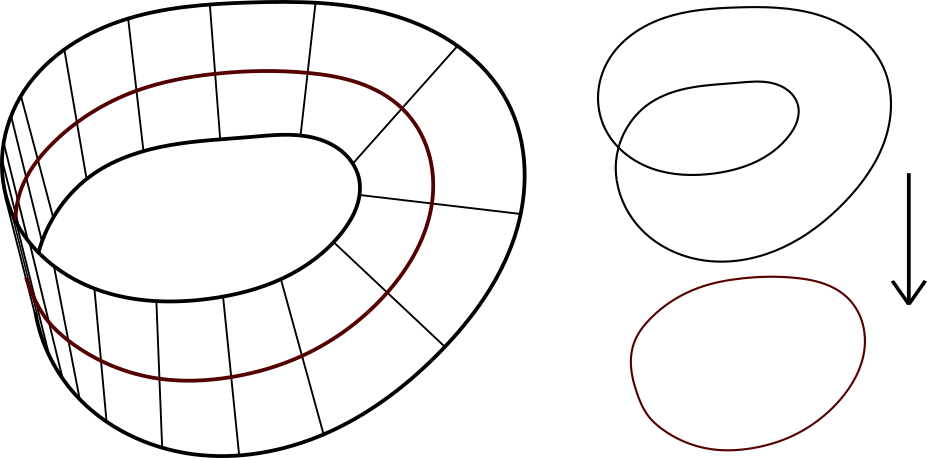
\includegraphics[width=.8\textwidth]{img/moebius.png}
    \caption{The Möbius-bundle over $S^1$ giving rise to a nontrivial covering over $S^1$ by assigning to each fiber the two possible orientations of that fiber.}\label{fig:moeb}
\end{figure}
The space $\BSO(n)$ classifies oriented vector bundles of rank $n$. Let $\t_n$ be the map $\BSO(n) \to \BO(n)$ which by postcomposition forgets orientation.
A lift of an orientable vectorbundle $V$ (represented by a map $M\to \BO(n)$) along $\t_n$ corresponds precicely to a choice of orientation for $V$. 
The map $\t_n$ is a partial double cover, since there are always exactly two possible orientations for a given orientable bundle.
The family of Maps $\t_n$ is compatible with stabilization, for this we just fix the usual orientation $\R^k$ to be the orientation of any trivial bundle. 
Therefore we obtain a colimit map $\t\colon \BSO \to \BO$ which by abstract nonsense is a fibration.\\
The tuple $(\BSO,\t)$ is now a tangential structure by above definition. 
A manifold $M$ admits this $\t$-structure, if its stable tangent bundle lifts along $\t$, i.~e. for some $K\in\N$ and all $k\geq K$ the $k$-times stabilized tangent bundle $TM\oplus \epsilon_k$ is orientable.
It is an elementary fact that $\mathfrak{o}(TM\oplus \epsilon_k) \to M$ is just the usual orientation double cover of $M$, so the choice of an orientation for $M$ makes up exactly to the choice of an orientation for some (and then all) $TM\oplus\epsilon_k$.
The example shows, that for $\t\colon \BSO \to \BO$ a manifold $M$ has a $\t$-structure if and only if it is orientable, and a $\t$-manifold is hence just a oriented manifold. \\
A more systematic way of obtaining interesting examples of $\theta$-structures comes from the \emph{Whitehead-tower} of $\BO$.
We denote it by 
\begin{equation*}
    \cdots \to \BO\langle k\rangle \to \cdots \to \BO\langle 2\rangle \to \BO\langle 1\rangle \to \BO\langle 0\rangle = \BO.
\end{equation*}
All the horizontal maps are fibrations, and the $k$-th stage is obtained from the one below by attaching cells killing the $k$-th homotopy group.
\begin{figure}
    \centering
    \includegraphics[width=\textwidth]{img/tikz/bott.pdf}
    \caption{Homotopy groups of $\BO,\BSO$, and $\BSpin$}\label{fig:bott}
\end{figure}
Due to the celebrated Bott periodicity theorem, the homotopy groups of the stable orthogonal group $\mathrm{O}$ are known and $8$-periodic (see \fref{fig:bott}).
From these, one obtains the homotopy groups of $\BO$ using the loopspace-suspension adjuncion in
\begin{equation*}
    \pi_{i+1}(\BO) = [S^{i+1},\BO] \cong [\Sigma S^i,\BO] \cong [S^i,\Omega\BO] \cong [S^i,\mathrm{O}] = \pi_i(O)
\end{equation*}
as well as the fact that $\B$ is a delooping.
The space $\BO$ has thus just the homotopy groups of $\mathrm{O}$ shifted up by one (see again \fref{fig:bott}), and is furthermore pathconnected.
Lifting a map, say the stable tangent bundle of a manifold, up by a stage is possible if the lifting obstructions for that stage vanishes.
We will take some time to elaborate that point and see how this construction generalizes the example of oriented bundles.
The fiber of the $k$-th fibration $\BO\langle k \rangle \to \BO\langle k -1 \rangle$ is an \emph{Eilenberg--MacLane-space} for the group $\pi_{k}(\BO)$ in degree $k$, which we denote $K(\pi_k(\BO),k)$ as is common.
Let $M$ be a manifold and $\hat{\st}\colon M\to \BO\langle k-1 \rangle$ a given lift of the stable tangent bundle, which we wish to lift one stage higher.
Denote by $M^{(i)}$ the $i$-skeleton of a CW-Decomposition of $M$, which since every smooth manifold admits a triangulation always exists.
We now wish to inductively solve the skeletal lifting problem
\begin{center}
    \begin{tikzcd}
        M^{(i+1)} \arrow[r, dashed] & \BO\langle k \rangle\arrow[d] \\
        M^{(i)} \arrow[u,hook]\arrow[ur]\arrow[r,"\hat{\st}"] & \BO\langle k-1 \rangle
    \end{tikzcd}
\end{center}
that asks whether we can extend the given lift on the $i$-skeleton to the $i+1$-skeleton.
Since the Fiber $K\big(\pi_k(\BO),k\big)$ is $k-1$-connected, there are no obstructions up until the $k-1$-skeleton of $M$.
The lifting obstruction from the $k-1$ to the $k$-skeleton is given by a certain cohomology class 
\begin{equation*}
    c\in H^{k}\Big(\BO\langle k -1 \rangle;\pi_k\big(K(\pi_k(\BO),k)\big)\Big) = H^{k}\big(\BO\langle k-1 \rangle;\pi_k(\BO)\big)
\end{equation*}
If then $\hat{\st}^\ast c$ vanishes, we obtain a lift to the $k$-skeleton of $M$. 
All higher homotopy groups of the fiber vanish, so from there on no further obstructions arise, and we get the desired lift on $M$.
Since Eilenberg--MacLane-spaces represent cohomology, we can alternatively think of the single obstruction $c$ as a (homotopy class of) map $\BO\langle k-1 \rangle \to K\big(\pi_k(\BO),k\big)$, which we will also denote $c$ in slight abuse of notation.
The dashed lift in
\begin{center}
    \begin{tikzcd}
        & \BO\langle k\rangle \arrow[d] & \\
        M \arrow[r,"\hat{\st}"]\arrow[ur,dashed] & \BO\langle k -1\rangle \arrow[r,"c"] & K\big(\pi_k(\BO),k\big)
    \end{tikzcd}
\end{center}
then exists, if and only of $\pi_k(c\circ\tau) = 0$.
We will jump frequently between these two viewpoints of the lifting obstruction in this work.
How does the Whitehead-tower tie into the discussed example?
Since $\pi_1(\BO)\cong \zz$ and $\BSO$ is pathconnected, the double cover $\BSO \to \BO$ is already the universal cover $\BO\langle 1 \rangle \to \BO$.
We have $H^1(\BO;\zz) \cong \zz$ by Hurewicz and excision, so the first universal Stiefel--Whitney-class $\overline{w}_1$ provides the unique obstruction class to orientability.
Similarly, the second universal Stiefel--Whitney-class $\overline{w}_2\in H^2(\BSO;\zz) = H^2(\BO;\zz) \cong \zz$ is the unique lifting obstruction against $\BO\langle 2 \rangle \to \BSO$.
\begin{defi}[Spin]
    A spin-structure on a manifold is a $\theta$-structure for the fibration $\t\colon \BSpin = \BO\langle 2\rangle \to \BO$. We call the $\theta$-manifolds of this tangential structure spin-manifolds.
\end{defi}
By the above, a manifold $M$ with stable tangent bundle $\st\colon M \to \BO$ is therefore orientable, iff $w_1(TM) = \st^\ast \overline{w}_1$ vanishes and \emph{spinnable} iff furthermore $w_2(TM) = \st^\ast \overline{w}_2$ vanishes aswell.\\
A surface $S$ is orientable if and only if it contains no Moebius-band.
Can we generalize this intuition to higherdimensional manifolds?
And what does a Spin-structure even entail geometrically?
We finish this section with such a geometric interpretation, which will be directly extracted from the obstruction theory point of view above.
\begin{thesislemma}\label{geomspin}
Let $M$ be a manifold. Then $M$ is orientable, if and only if for any continuous $\iota\colon S^1 \to M$ the restriction $\st\circ \gamma$ of the stable tangent bundle is trivializable.
    If $\dim(M)\geq 3$, $M$ is furthermore spinnable, if and only if additionally for any surface $S$ and continuous map $\iota\colon S\to M$ the restriction $\st\circ \iota$ is trivializable. 
\end{thesislemma}
\pagebreak{} % ugly but neccesary, for some reason prf sticks to lem
\prf
    Let $[X]\in H_d(X;\zz)$ denote the $\zz$ fundamental class of a $d$-dimensional manifold $X$. 
    The family
    \begin{equation*}
        \big\{ \iota_\ast [S_i] \:\big\vert\: \iota\colon S_i \to M, S_i \text{ compact manifold of dim } i \big\}
    \end{equation*}
    obviously generates $H_i(M;\zz)$.
    We may thus test vanishing of the Stiefel--Whitney-classes of $M$ on this family.
    Via naturality
    \begin{equation*}
        \langle w_i(TM), \iota_\ast[S_i] \rangle = \langle \iota^\ast w_i(TM), [S_i] \rangle = \langle w_i(\iota^\ast TM),[S_i]\rangle 
    \end{equation*}
    so the $i$-th Stiefel Whitney class of $M$ vanishes if and only if it vanishes restricted along all $S_i \to M$.
    $[S^1,\BO]$ has only two elements, so vanishing of the first Stiefel--Whitney-class already implies trivializability of a bundle over $S^1$.
    This finishes the proof of the first part, since $S^1$ is the only one dimensional manifold.\\
    For the second part, note that it suffices looking at only orientable surfaces $S \to M$. 
    Any orientable rank $\geq 3$ bundle over a oriented surface is already trivial if its second Stiefel--Whitney-class vanishes.
    This is due to the following observation:
    Cutting out a disk $D\cong D^2$ from a surface $S$ we may retract the remains to a wedge of circles, the $1$-skeleton of $S$.
    Over this $1$-skeleton, the bundle trivializes due to the vanishing of $w_1$.
    Since $D\whe \{\ast\}$ also there the bundle trivializes and we thus obtain all rank $d$ vectorbundles over the surface by a clutching map $S^1 \to SO(d)$.
    Now for $d\geq 3$ we have $\pi_1(\mathrm{SO}(d)) \cong \pi_2(\BSO) \cong \zz$, so vanishing of $w_2$ implies trivializability.
\endprf
For manifolds of dimension $1$ the lemma of course holds vacuously, but in dimension $2$ the relationship is knavish.
Whilst the tangent bundle of $S^2$ is famously nontrivial due to the hairy-ball-theorem, it has trivial Stiefel--Whitney-classes, since embedding $S^2$ into $\R^3$ gives a decomposition $TS^2 \oplus \underline{\R} \to T\R^3$ where $\underline{\R} = S^2\times\R$ is the trivialized normal bundle of the embedding.
Hence $S^2$ is spinnable, but its tangent bundle pulled back along the identity is nontrivial, violating the lemma.
The violation is not severe however, any orientable surface $S$ is spinnable, since if its genus is larger than $0$, we have $\pi_2(S) = 0$ removing $w_2$.\\
To strenghten the geometrical picture further, we pass from arbitrary maps to embeddings.
\begin{thesisprop}\label{orgeom}
    Let $M$ be a manifold. Then $M$ is orientable if $\iota^\ast TM$ is trivial for every embedding $\iota\colon S^1 \to M$.
\end{thesisprop}
\prf
    For $\dim(M) = 1$, the statement is easily verified by taking $\id_{S^1}$ as the embedding.
    Else, note that the homotopy class of any map $f\colon S^1 \to M$ contains a smooth representative by the Whitney approximation theorem.
    With $\dim(M)\geq 3$, this smooth representative may be taken to be an embedding by the Whitney embedding theorem, and the proposition follows instantly from \ref{geomspin}.
    In dimension $2$, one can use the classification of surfaces to directly see that every nonorientable surface contains a Möbius-band.
\endprf
This is best visualized in the following example:
A half equator $S_+^1 \hookrightarrow S^2$ maps onto a $S^1 \hookrightarrow \RP^2$ under the canonical projection $S^2\to \RP^2$. 
The normal bundle $\nu$ of this embeddeding $\iota\colon S^1\hookrightarrow \RP^2$ is the nontrivial Moebius-bundle, and the tangent direction is trivial.
Thus in total the restriction of the tangent bundle of $\RP^2$ along $\iota$ has $w_1(\iota^\ast T\RP^2) = w_1(\nu) \neq 0$ showing that it is nontrivial and $\RP^2$ is nonorientable!
\begin{thesisprop}\label{moregeomspin}
    Let $M$ be a simply connected manifold of dimension $d\geq 5$. Then $M$ is spinnable, if $\iota^\ast TM$ is trivial for every embedding $\iota\colon S^2 \to M$.
\end{thesisprop}
\prf
    Since $M$ is simply connected, $w_1(M) = 0$ and by Hurewicz every element in $H_2(M)$ comes from a continuous map $S^2 \to M$.
    With $d\geq 5 = 2* 2 + 1$ we may again use the Whitney approximation and embedding theorem to deform any such continuous map to an embedding. 
    Then as another application of \ref{geomspin} the proof is done.
\endprf

